\chapter{Desarrollo de la Solución}
\label{sec:desarrollo}

\section[Proceso de Desarrollo]{Proceso de Desarrollo}

\subsection{Versionado de código}

\subsection{Integración Continua}

\subsection{Tests}

\section[Núcleo]{Núcleo}

El núcleo se encarga de administrar los datos no sensibles de los alumnos y sus materias cursadas, las inscripciones, planes de estudio con sus créditos, recorrido obligatorio y recomendado de inscripciones, entre otros.
El núcleo tiene la capacidad de servir dichos datos para que sean consumidos por los usuarios que tengan los permisos correspondientes.
Los usuarios tienen permisos asignados que corresponden con la carrera a la que pertenecen, que les permiten consultar datos de dicha carrera. 






\begin{figure}[h!]
  \centering
    
\includegraphics[scale=0.5]{images/nucleo/nucleo-fondoblanco.png}
  \captionof{figure}{Logo del Núcleo}
  \label{fig:django}
\end{figure}

\subsection{Tecnologías}

El Núcleo fue desarrollado con Python 3.6, usando el framework web Django en su versión 3.0.
Django incluye un administrador (django-admin) que genera automáticamente los listados, la creación, la edición y el borrado de los modelos desarrollados. Además, trae un sistema de autenticación de usuarios que facilita la tarea de autorizar usuarios a través de permisos.
Se eligió django-rest-framework para crear una API REST para que otros servicios puedan consultar o crear datos.
Usando django-rest-framework-simplejwt, se implementó JWT. Es decir, todo servicio que quiera acceder a los datos tendrá que pedir un token. Si éste está habilitado para consumir datos, se le proveerá de dicho token.

\subsection{Administración de los datos}

Los usuarios que tengan permiso para ingresar al Administrador, pueden hacerlo mediante una pantalla de Login como muestra la figura ~\ref{fig:nucleo-login}.
Una vez ingresados, pueden ver la pantalla principal del administrador, como muestra la figura ~\ref{fig:nucleo-home}, donde tienen diferentes menús para utilizar los datos. Tienen acceso a diferentes listados (figura ~\ref{fig:nucleo-listado}), creación, edición y borrado (figura ~\ref{fig:nucleo-edicion}).
Los usuarios tienen también la posibilidad de importar planillas de datos (figura ~\ref{fig:nucleo-importador}).

\subsubsection{Usuarios y permisos}

Para resolver la autenticación y autorización en el administrador de contenidos, se usó el sistema de autenticación que viene embebido en Django.
Este sistema provee una manera de asignar permisos a usuarios específicos o grupos de usuarios. Estos permisos se dividen en:
\begin{outline}
    \1 El acceso a ver objetos está limitado a los usuarios que tengan los permisos \textit{view} o \textit{change}.
    \1 El acceso a ver los formularios para agregar elementos, está limitado a los usuarios que tengan el permiso \textit{add} para ese tipo de objetos.
    \1 El acceso a ver los listados, ver los formularios de edición y la posibilidad de editar, están limitados a los usuarios que tengan el permiso \textit{change} para ese objeto en particular.
    \1 El acceso a eliminar un objeto está limitado a los usuarios que tengan el permiso \textit{delete}.
\end{outline}

\subsubsection{Grupos de usuarios}

Django provee una forma de categorizar usuarios a los que se les puede aplicar permisos llamado \textit{grupo}. Un usuario puede pertenecer a muchos grupos.
Un usuario que pertenezca a un grupo, automáticamente tiene los permisos asignados a dicho grupo.
Otra particularidad de esto, además de los permisos, es que pueden servir para extender las funcionalidades. Por ejemplo, si quisiera que un grupo fuese "Usuarios de LIDS", podría asignarle a ese grupo la carrera "LIDS" para que sólo pudieran ver datos relacionados a su carrera y no a otras.


\subsection{Importadores}

En el caso que los usuarios tengan la necesidad de importar los datos a través de planillas, se realizaron diferentes importadores para esta tarea (~\ref{fig:nucleo-importador}).
Estos importadores son:
\begin{outline}
\2 Carreras
\2 Planes de estudio con sus materias
\2 Prerrequisitos obligatorios y recomendados de materias
\2 Alumnos con sus datos personales
\2 Materias cursadas por alumnos
\2 Inscripciones a materias
\end{outline}

\subsection{API}

Se diseñó una API para consultar datos a través de distintas URIs (tabla ~\ref{tab:tabla_api}), para las cuales se necesita de un token (tabla ~\ref{tab:tabla_token}).
Dicho token es de la forma:

\textit{eyJ0eXAiOiJKV1QiLCJhbGciOiJIUzI1NiJ9.} \break 
\textit{eyJ0b2tlbl90eXBlIjoiYWNjZXNzIiwiZXhwIjoxNTg5Mjk2NjAyLCJ}\break 
\textit{qdGkiOiJhMTAzMmI2YzdiN2Y0ZjlkODc5NzI0NGViZTQxYTk5YSIsInV}\break 
\textit{zZXJfaWQiOjEsImNhcnJlcmFzIjpbIlciXSwiY2FycmVyYXNfbGFiZWwi} \break \textit{OltbIlciLCJMaWNlbmNpYXR1cmEgZW4gRGVzYXJyb2xsbyBkZSBTb2Z0d2}\break 
\textit{FyZSJdXSwidXNlcm5hbWUiOiJhZG1pbiJ9}.\break 
\textit{xWWi-sDFQ6I-CK0xC7tmkTw1mXRmMhFFse6\_qnKBiaE}

\break
El \textit{Header} del token tiene la siguiente información:
\begin{lstlisting}[language=json,firstnumber=1]
{
"typ": "JWT",
"alg": "HS256"
}
\end{lstlisting}
\break
Para el caso del \textit{Payload}, se tiene la siguiente información indicando precisamente qué carreras puede consultar el usuario:
\begin{lstlisting}[language=json,firstnumber=1]
{
  "token_type": "access",
  "exp": 1589296602,
  "jti": "a1032b6c7b7f4f9d8797244ebe41a99a",
  "user_id": 1,
  "carreras": [
    "W"
  ],
  "username": "admin"
}
\end{lstlisting}

\subsubsection{Ejemplo de pedido}
Si quisiera saber qué materias hay dentro de una carrera en un plan determinado, deberia hacer de la siguiente manera:

\begin{lstlisting}[language=bash]
GET 'https://url.del.nucleo/api/carreras/W/planes/2015/'
--header Authorization: Bearer <token>
\end{lstlisting}

El resultado tendrá la siguiente forma:

\begin{lstlisting}[language=json,firstnumber=1]
[{
        "id": 54,
        "materia": "Taller de Trabajo Intelectual",
        "plan": 2015,
        "nucleo": "",
        "creditos": 4,
        "area": "Taller",
        "codigo": "00751"
    },
    ...
]
\end{lstlisting}

\begin{figure}[h!]
  \centering
    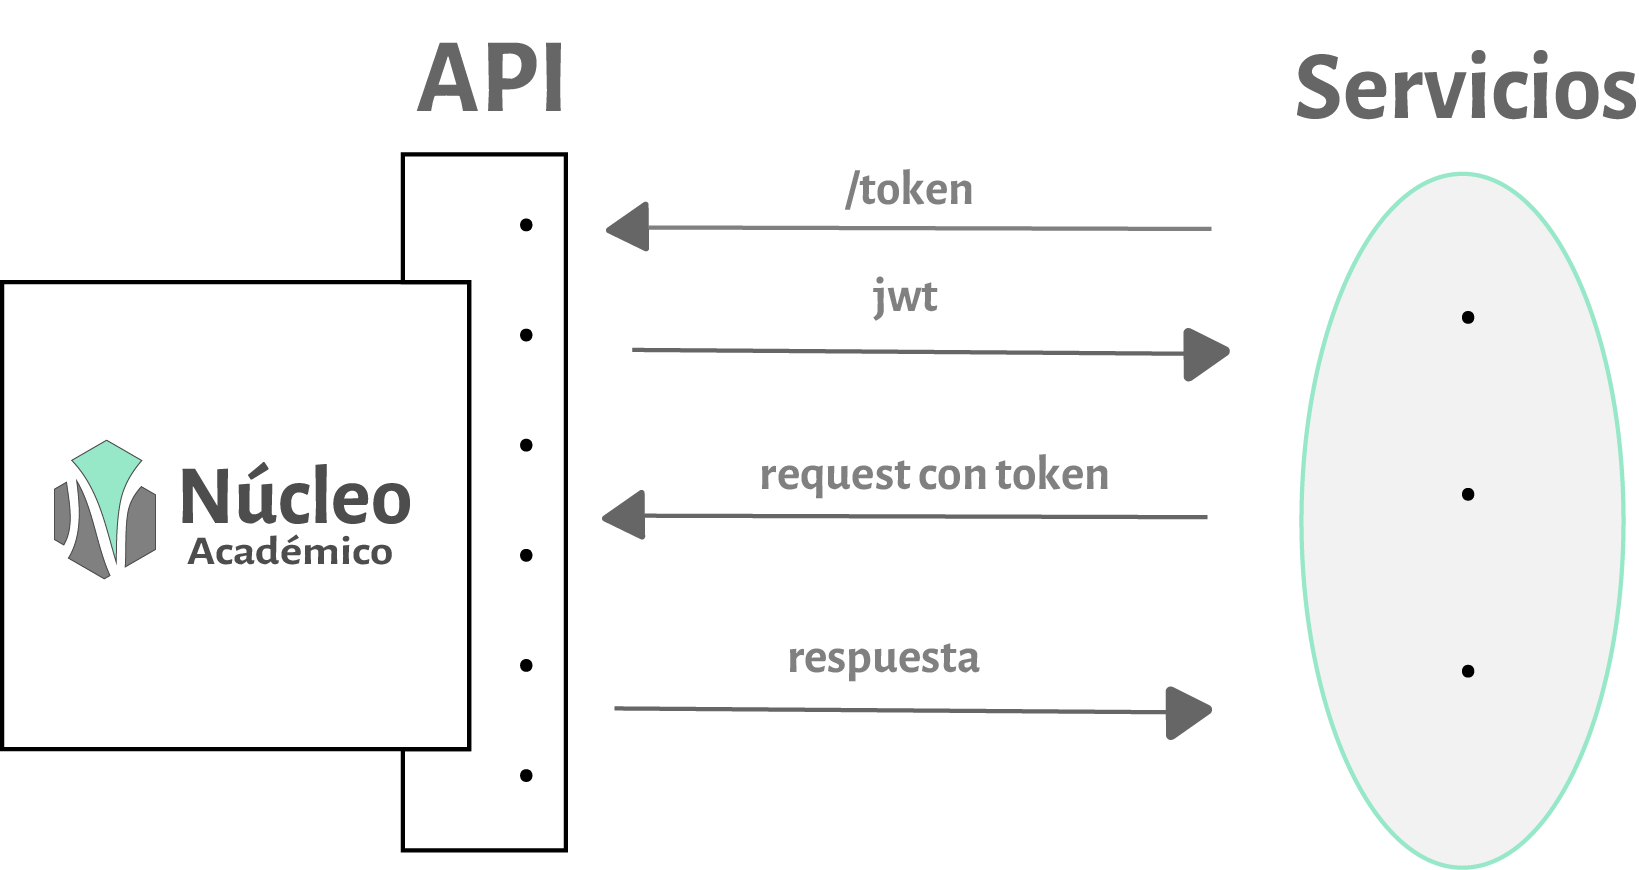
\includegraphics[scale=0.8]{images/nucleo/jwt.png}
  \captionof{figure}{Funcionamiento del pedido de token y posteriores requests}
  \label{fig:nucleo-jwt}
\end{figure}


\subsection{Deploy}

Docker, nginx, base de datos

\section[Análisis de Datos]{Análisis de Datos}

Para poder obtener información relevante de las carreras, materias y alumnos, se debe hacer un análisis de los datos recopilados históricamente.

Si bien el núcleo provee una gran cantidad de datos, éstos necesitan una manipulación, procesamiento y una limpieza para que puedan ser analizados.

El objetivo principal de este módulo es de la obtención de los datos mediante una API Rest, la manipulación y el procesamiento de esos datos. Una vez terminado este proceso, sirve los resultados mediante una API Rest, que es consumida por un tercero para su visualización.

\subsection{Especificaciones}

El módulo de análisis de datos está construido con Python 3.6. El análisis de los datos se hizo con Pandas y los resultados son servidos gracias a Flask a través de una API REST.


El siguiente gráfico muestra el rol de este módulo y su funcionamiento con respecto al núcleo

\begin{figure}[h!]
  \centering
    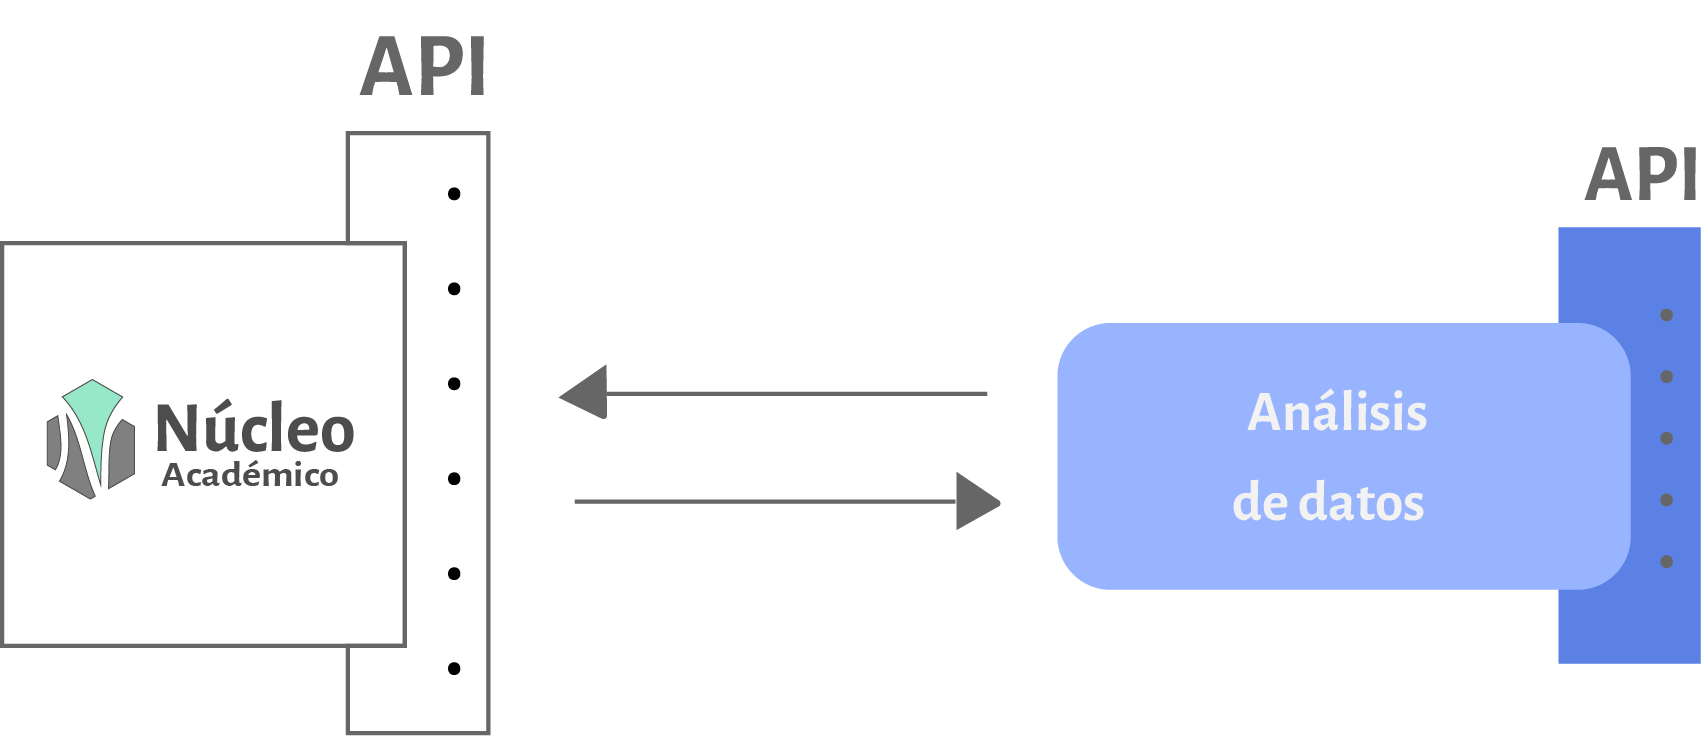
\includegraphics[scale=0.8]{images/analisis-datos/analisis-datos.png}
  \captionof{figure}{Obtención de datos a través del núcleo}
  \label{fig:django}
\end{figure}

\subsection{Obtención de los datos}

Los datos son obtenidos a través de pedidos a la API del Núcleo. Estos datos llegan en forma de JSON y son transformados a DataFrame o Series (estructuras de datos de Pandas). 

Dado que los datos llegan de forma de recursos independientes, la mayor parte de los análisis requieren que estos datos sean unidos gracias a las funcionalidades de los DataFrames (de forma similar a los join de SQL).

\subsection{Análisis}

Una vez terminados los procesos de obtención, limpiado y union de los datos, se empieza el proceso de análisis.

Se realizaron análisis de diferentes magnitudes, basado en la cantidad de procesamiento que requieren. 
\subsubsection{Análisis sobre materias}

\paragraph{Datos basicos históricos} \mbox{}\\
URI: /materias/<cod\_materia>/basicos \\
Parámetros opcionales: inicio: yyyy-mm-dd, fin: yyyy-mm-dd, carrera: codigo de la carrera. \\
Dada una materia, analiza cuántos aprobaron, cuántos desaprobaron, cuántos quedaron ausentes y cuántos faltan aprobarla dentro de un período de tiempo.

\paragraph{Detalle de aprobación}\mbox{}\\
URI: /materias/<cod\_materia>/detalle-aprobados \\
Parámetros opcionales: inicio: yyyy-mm-dd, fin: yyyy-mm-dd, carrera: codigo de la carrera. \\
Dada una materia, dice el detalle de aprobados. Teniendo en cuenta la forma de aprobación. Las formas de aprobacion son:

>> Formas de aprobación

\paragraph{Dispersión de notas}\mbox{}\\

URI: /materias/<cod\_materia>/dispersion-notas \\
Parámetros opcionales: inicio: yyyy-mm-dd, fin: yyyy-mm-dd, carrera: codigo de la carrera. \\
Dada una materia, se hace un análisis de la dispersión de las notas dentro de un período. Teniendo en cuenta alumnos, sus notas y el promedio de ese alumno.

\paragraph{Número de recursantes}\mbox{}\\
URI: /materias/<cod\_materia>/recursantes \\
Parámetros opcionales: inicio: yyyy-mm-dd, fin: yyyy-mm-dd, carrera: codigo de la carrera. \\
Dada una materia, analiza qué alumnos son recursantes y cuantas veces


\subsubsection{Análisis sobre alumnos}

\paragraph{Porcentaje de aprobación por área}\mbox{}\\

URI: /alumnos/<legajo>/porcentajes-areas \\

Parámetros adicionales: carrera, inicio, fin, plan \\

Dado un alumno, se hace un análisis de los porcentajes de aprobación que tiene con respecto a las diferentes áreas de la carrera y el plan que se está analizando, dentro del período elegido.

Cada carrera tiene sus propias áreas. En particular, y tomado a forma de ejemplo, las áreas de la Licenciatura en Informática son:

\begin{table}[!htbp]
    \centering
    \makegapedcells
    \begin{tabular}{|c|c|}
    \hline
    Nombre \\ \hline
    Programación \\ \hline
    Sistemas Informáticos \\ \hline
    Procesos Informáticos\\ \hline
    Desarrollo de Software \\ \hline
    Teoría de la Computación \\ \hline
    \end{tabular}
    \caption{Áreas de la Licenciatura en Informática}
    \label{tab:tabla_areas}
\end{table}

\paragraph{Porcentaje de aprobación por núcleo}\mbox{}\\

URI: /alumnos/<legajo>/porcentajes-nucleos \\

Parámetros adicionales: carrera, inicio, fin, plan \\

Dado un alumno, se hace un análisis de los porcentajes de aprobación que tiene con respecto a los diferentes núcleos de la carrera y el plan que se está analizando, dentro del período elegido.

Cada carrera tiene sus propias núcleos. En particular, y tomado a forma de ejemplo, los núcleos de la Licenciatura en Informática son:

\begin{table}[!htbp]
    \centering
    \makegapedcells
    \begin{tabular}{|c|c|}
    \hline
    Código & Nombre \\ \hline
    I & Introductorio \\ \hline
    B & Básico\\ \hline
    A & Avanzado \\ \hline
    C & Complementario/Orientativo \\ \hline
    \end{tabular}
    \caption{Núcleos de la Licenciatura en Informática}
    \label{tab:tabla_nucleos}
\end{table}


\paragraph{Notas}\mbox{}\\

URI: /alumnos/<legajo>/notas \\

Parámetros adicionales: carrera, inicio, fin, plan \\

Dado un alumno, se obtienen las diferentes notas que tuvo a lo largo de sus cursadas.

\paragraph{Porcentaje de avance de carrera}\mbox{}\\

URI: /alumnos/<legajo>/porcentaje-carrera \\

Parámetros adicionales: carrera, inicio, fin, plan \\

Dado un legajo de alumno, se realiza un análisis para determinar el porcentaje de avance de la carrera, según el plan que se analice. Dado que cada plan tiene una cantidad distinta de materias, este dato cambia según el plan que se analice.

\paragraph{Promedio por períodos}\mbox{}\\

URI: /alumnos/<legajo>/scores \\

Parámetros adicionales: carrera, inicio, fin, plan \\

Dado un alumno, se calcula cuál fue su **score** por cada período. Es decir, su rendimiento semestral. 

El **score** se calcula sacando un promedio de sus notas en un semestre. Las materias que sólo se distinguen entre "Aprobado" y "Desaprobado" y no disponen de una nota, se les asigna una nota para sacar este promedio.
Las materias con nota "Aprobado" son consideradas como un 7, y las materias con nota "Desaprobado" son consideradas como un 3.

Entonces, el **score** no es un promedio preciso, sino una estipulación de lo que fué su rendimiento en ese período.

Este score es útil para analizar el rendimiento de un alumno y puede servirle a las carreras para tomar decisiones tempranas.

\subsubsection{Análisis sobre carreras}

\paragraph{Cantidad de alumnos por semestre}\mbox{}\\

URI: /carreras/<carrera>/alumnos \\

Dada una carrera, se obtiene un listado de cantidad de inscriptos por semestre


\paragraph{Datos generales por cohorte}\mbox{}\\

URI: /carreras/<carrera>/cantidades-alumnos \\

Dada una carrera, se obtiene un listado de inscriptos, cursantes, graduados y postulantes por cohorte.


\paragraph{Ingresantes por cohorte}\mbox{}\\

URI: /carreras/<carrera>/cantidades-ingresantes \\

Dada una carrera, se obtiene la cantidad de ingresantes separadas por año.


\paragraph{Cantidad de cursantes actual}\mbox{}\\

URI: /carreras/<carrera>/cursantes-actual \\

Dada una carrera, se obtiene la cantidad de cursantes actual.


\paragraph{Cantidad de ingresantes actual}\mbox{}\\

URI: /carreras/<carrera>/ingresantes-actual \\

Dada una carrera, se obtiene la cantidad de ingresantes.


\paragraph{Cantidad total de graduados} \mbox{}\\

URI: /carreras/<carrera>/graduados-total \\

Dada una carrera, se obtiene el total de graduados.


\paragraph{Dispersión de scores y promedios}\mbox{}\\
URI: /carreras/<carrera>/dispersion-score-promedio \\

El objetivo de este análisis es el agrupar alumnos en base al score y al promedio. Mostrando grupos de interés sobre los cuales se podrán implementar acciones específicas.

\paragraph{Materias Traba}\mbox{}\\

URI: /carreras/<carrera>/materias-traba \\

Dada una carrera, se quiere analizar qué materias son las que traban a los alumnos. 
Para poder realizar este análisis, se necesitaron los siguientes datos:
\begin{outline}
\1 Índice de aprobación de una materia (cantidad de aprobados / cantidad total de cursantes).
\1 Cuántas materias obligatorias dependen de ella.
\end{outline}

Luego de calcular estos datos materia por materia, se calcula un score. Este score determina qué materia puede llegar a trabar la carrera de un alumno.

\begin{align*}
  Score = IndiceAprobacion * CantidadObligatoriasDependientes\\
\end{align*}

Es decir, que una materia que tiene un porcentaje de aprobación del 75\% y 10 materias que son obligatorias y dependen de ésta para ser cursadas, tendrá un score de 7.5 (0.75 * 10).



\section[Visualización de los datos analizados]{Visualización de los datos analizados}

Si bien los datos ya fueron a analizados, se necesitó una forma de visualizarlos de forma gráfica. Por esta razón surgió la necesidad de crear una nueva aplicación independiente del núcleo y del análisis de datos.

Esta nueva aplicación obtuvo el nombre de Seguimiento Académico, y este es su logo:

\begin{figure}[h!]
  \centering
    
\includegraphics[scale=0.5]{images/seguimiento-academico/seguimiento-academico-blanco.png}
  \captionof{figure}{Logo de la aplicación de Seguimiento Académico}
  \label{fig:seguimiento-academico-logo}
\end{figure}

Su objetivo principal es recolectar los datos analizados y mostrarlos de forma gráfica, dependiendo de los permisos que tenga el usuario que realiza el pedido.
Estos datos se desprenden del módulo de análisis, y se agrupan de la siguiente manera:

\begin{outline}
\2 Datos sobre carreras.
\2 Datos sobre materias.
\2 Datos sobre alumnos.
\end{outline}

Cada uno de estos grupos de datos tiene su propia pantalla de tipo reporte, donde el usuario ingresa los parámetros necesarios para cada reporte.


\subsection{Especificaciones}

Seguimiento Académico esta construido con React 16.8 y se usó la libreria recharts para generar gráficos. Además, se uso el framework Material UI para el renderizado de elementos de la interfáz de usuario y diferentes tablas.
Este módulo realiza pedidos a la aplicación de análisis de datos, los cuales tienen que tener su correspondiente token para ser aceptados.
Cuando un usuario ingresa, se hace una autenticación con el núcleo. Esta autenticación tiene como resultado un token, y éste será utilizado para realizar todos los pedidos de datos correspondientes.

El siguiente gráfico muestra el rol de este módulo y su funcionamiento con respecto al de análisis de datos y al núcleo.

\begin{figure}[h!]
  \centering
    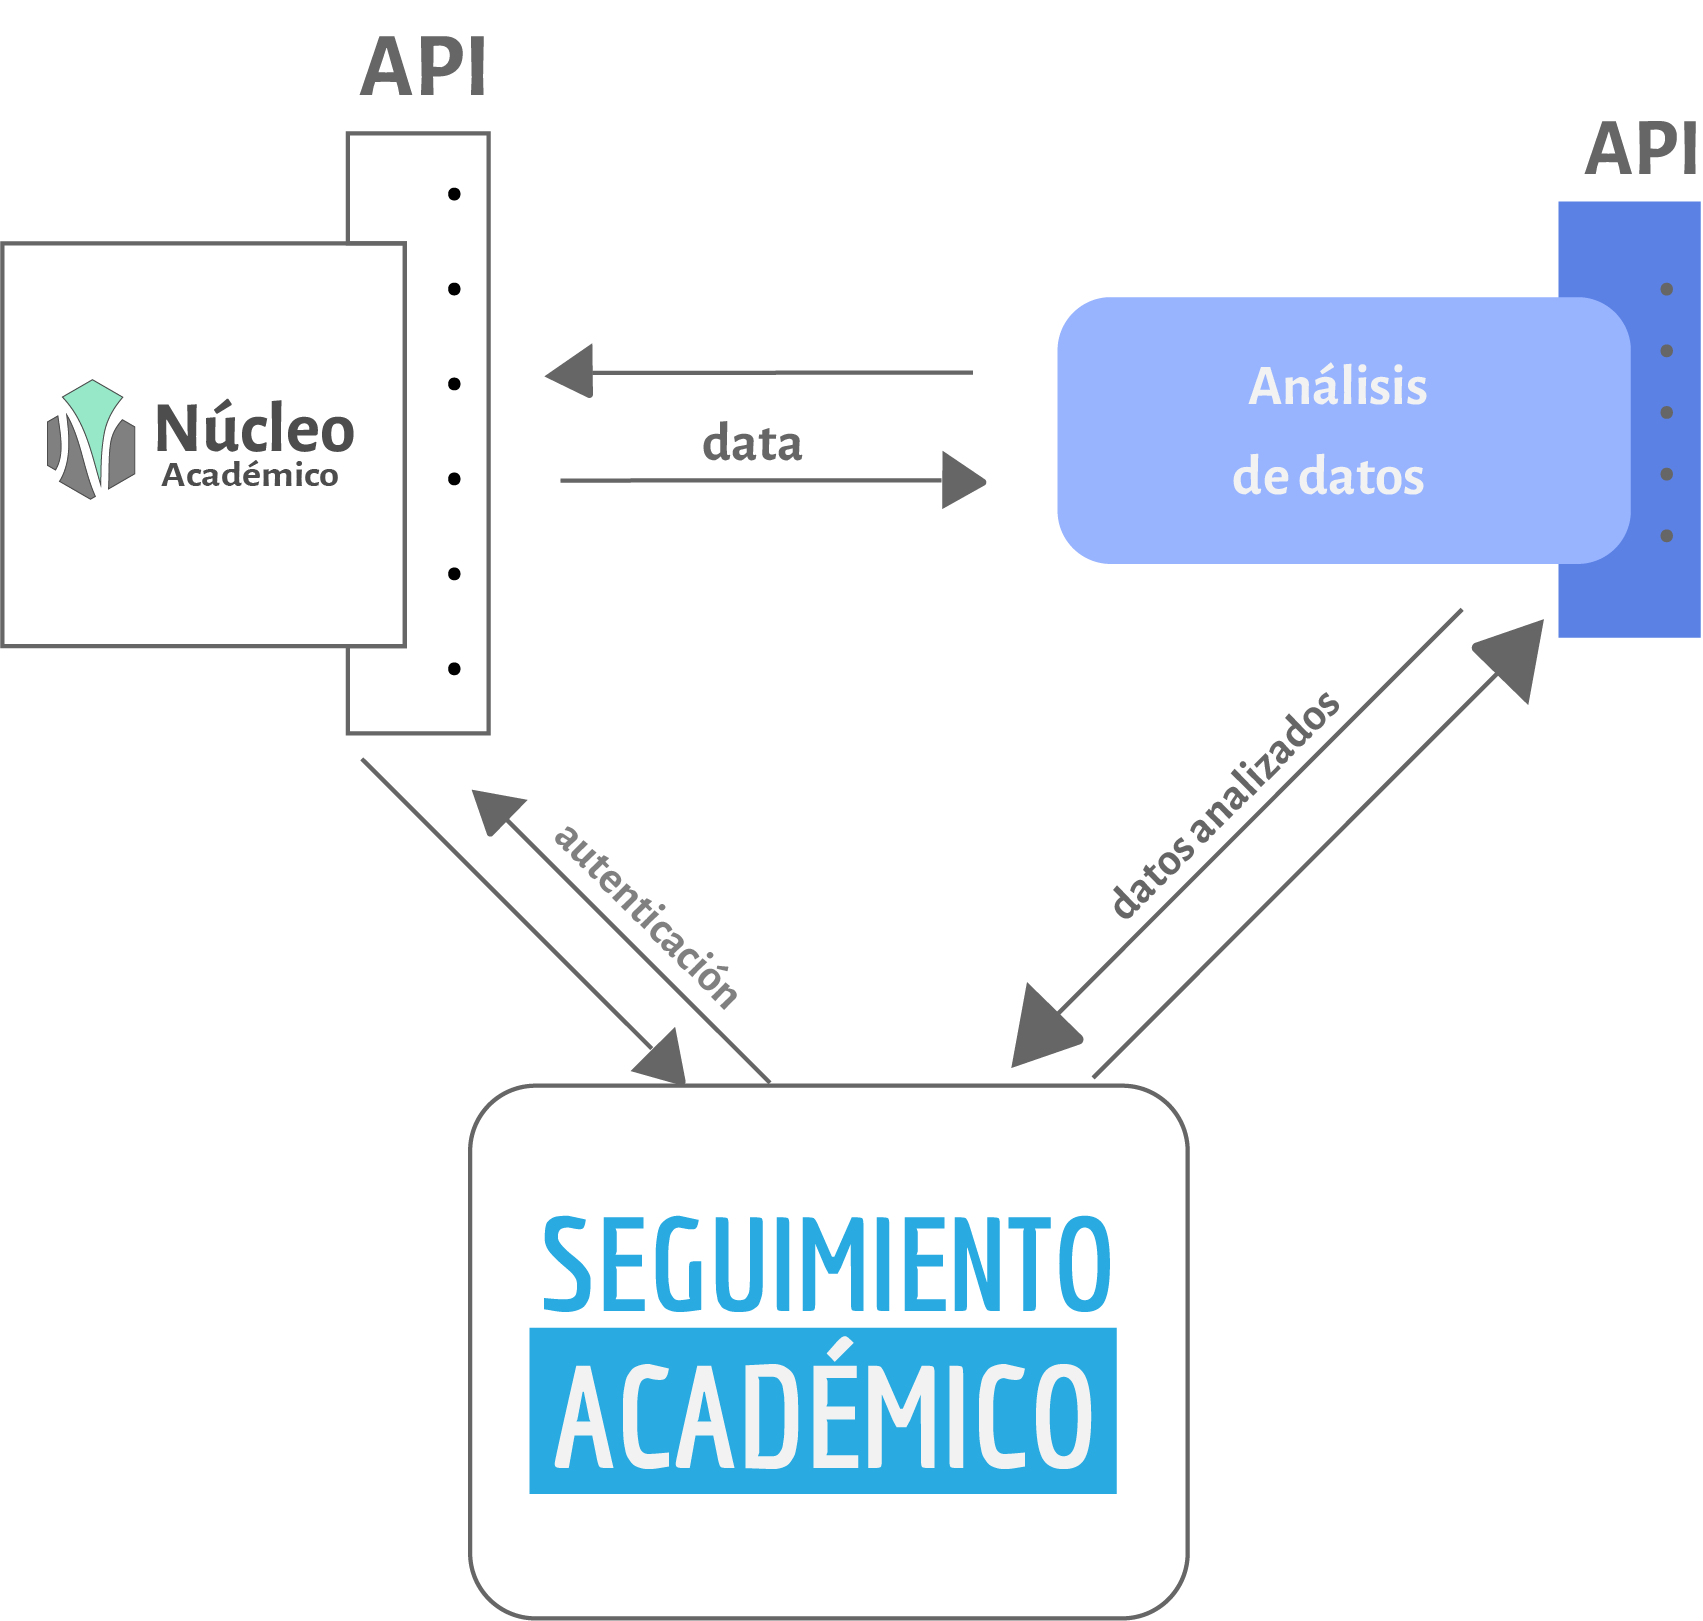
\includegraphics[scale=0.8]{images/seguimiento-academico/flow-seguimiento-academico.png}
  \captionof{figure}{Obtención de datos a través del núcleo}
  \label{fig:analisis-datos}
\end{figure}

\subsection{Obtención de los datos}

Los datos son obtenidos a través de pedidos a la API del módulo de análisis de datos. Estos datos llegan como JSON y son procesados para ser mostrados de forma correcta.


\subsection{Visualización de datos}

La aplicación Seguimiento Académico tiene 5 pantallas principales:
\begin{outline}
 \1 Login ().
 \1 Home ()
 \1 Reporte de Carrera ()
 \1 Reporte de Materia ()
 \1 Reporte de Alumno ()
\end{outline}


Hablar de las pantallas principales, hacer referencia a los anexos donde van a estar LOGIN, Home, Form de carrera, form de materia y form de alumno.

\subsubsection{Visualización por carrera}

\paragraph{Cantidad actual de cursantes} \mbox{}\\
Widget

\begin{figure}[!htbp]
  \centering
    
\includegraphics[scale=0.4]{images/seguimiento-academico/sa-cursantes.png}
  \captionof{figure}{Cantidad de cursantes}
  \label{fig:sa-cursantes}
\end{figure}

\paragraph{Cantidad actual de ingresantes} \mbox{}\\
Widget

\begin{figure}[!htbp]
  \centering
    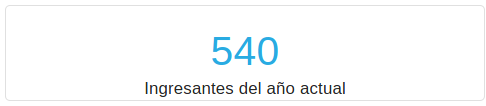
\includegraphics[scale=0.4]{images/seguimiento-academico/sa-ingresantes.png}
  \captionof{figure}{Cantidad de ingresantes}
  \label{fig:sa-ingresantes}
\end{figure}

\paragraph{Cantidad total de graduados} \mbox{}\\
Widget

\begin{figure}[!htbp]
  \centering
    
\includegraphics[scale=0.4]{images/seguimiento-academico/sa-graduados.png}
  \captionof{figure}{Cantidad de graduados}
  \label{fig:sa-graduados}
\end{figure}

\paragraph{Dispersión de alumnos} \mbox{}\\
Grafico de dispersión

\begin{figure}[!htbp]
  \centering
    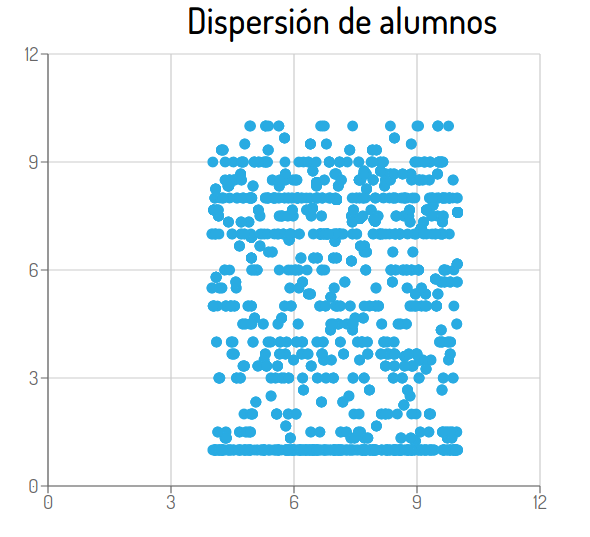
\includegraphics[scale=0.4]{images/seguimiento-academico/sa-dispersion.png}
  \captionof{figure}{Gráfico de dispersión}
  \label{fig:sa-dispersion}
\end{figure}

\paragraph{Cantidad de ingresos por semestre} \mbox{}\\
Grafico de area

\begin{figure}[!htbp]
  \centering
    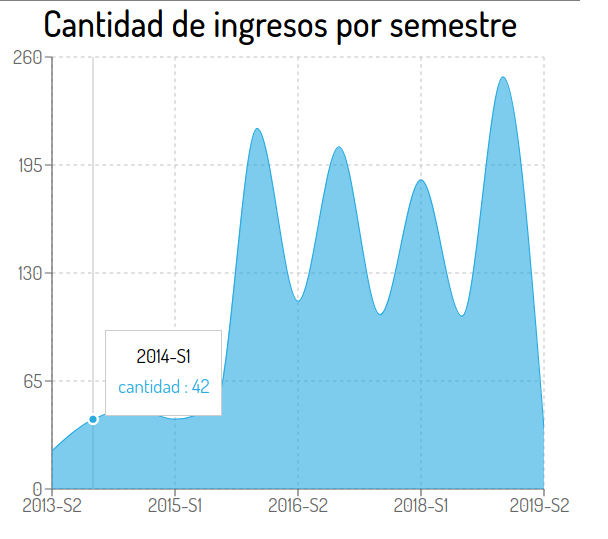
\includegraphics[scale=0.4]{images/seguimiento-academico/sa-ingresossemestre.png}
  \captionof{figure}{Ingresos por semestre}
  \label{fig:sa-ingresos-semestre}
\end{figure}

\paragraph{Alumnos por cohorte} \mbox{}\\
Tabla, CONEAU

\begin{figure}[!htbp]
  \centering
    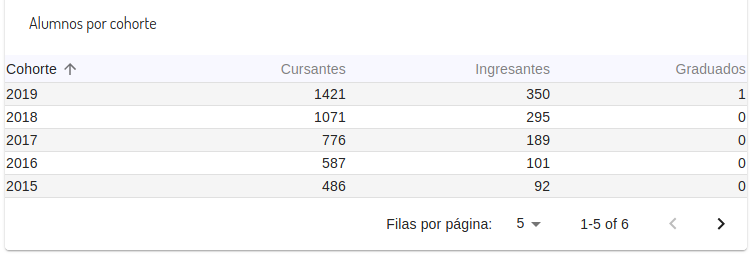
\includegraphics[scale=0.4]{images/seguimiento-academico/sa-alumnos-cohorte.png}
  \captionof{figure}{Tabla de alumnos por cohorte}
  \label{fig:sa-alumnos-cohorte}
\end{figure}

\paragraph{Ingresantes por cohorte} \mbox{}\\
Tabla, CONEAU

\begin{figure}[!htbp]
  \centering
    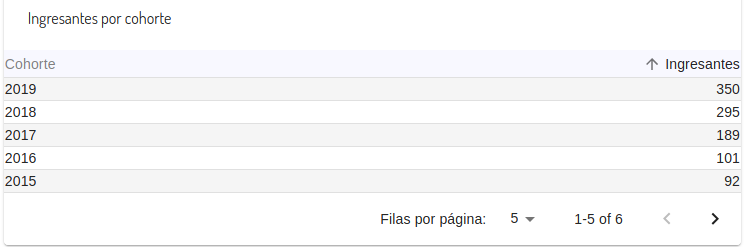
\includegraphics[scale=0.4]{images/seguimiento-academico/sa-ingresantes-cohorte.png}
  \captionof{figure}{Tabla de ingresantes por cohorte}
  \label{fig:sa-ingresantes-cohorte}
\end{figure}


\subsubsection{Visualización por materia}

Hablar del form y hacer referencia al anexo

\paragraph{Estadísticas básicas de materia} \mbox{}\\
Grafico de barras

\begin{figure}[!htbp]
  \centering
    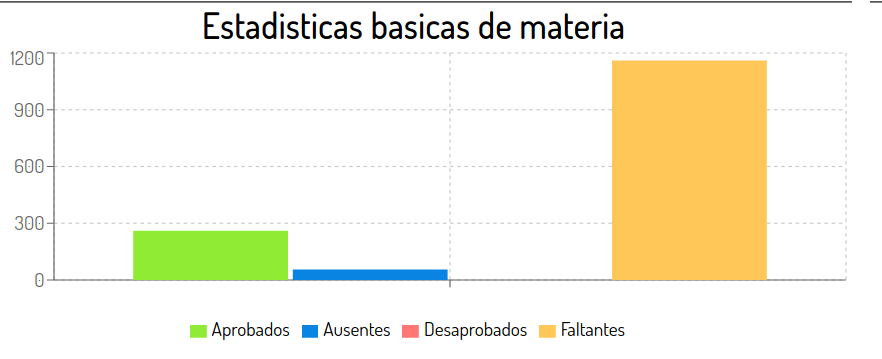
\includegraphics[scale=0.4]{images/seguimiento-academico/sa-datosbasicos.png}
  \captionof{figure}{Estadísticas básicas de la materia}
  \label{fig:sa-datos-basico}
\end{figure}

\paragraph{Detalle de aprobación} \mbox{}\\
Grafico de barras

\begin{figure}[!htbp]
  \centering
    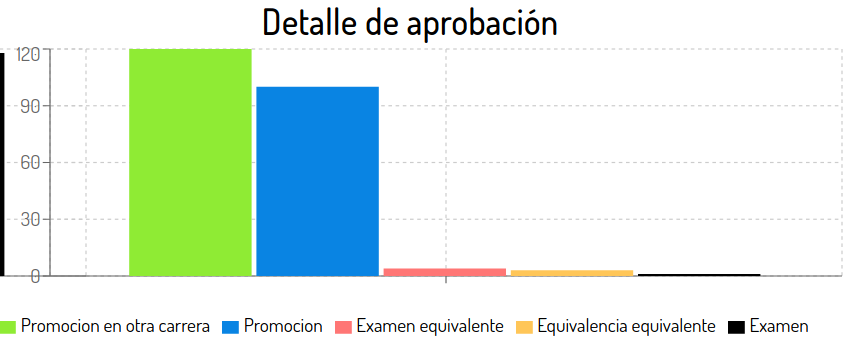
\includegraphics[scale=0.4]{images/seguimiento-academico/sa-detalleaprobacion.png}
  \captionof{figure}{Detalle de aprobación de la materia}
  \label{fig:sa-detalle-aprobacion}
\end{figure}

\paragraph{Dispersión de notas con respecto al promedio} \mbox{}\\
Grafico de dispersion

\subsubsection{Visualización por alumno}

\paragraph{Porcentaje de carrera} \mbox{}\\
Widget

\paragraph{Porcentajes de aprobación por área} \mbox{}\\
Radar

\begin{figure}[!htbp]
  \centering
    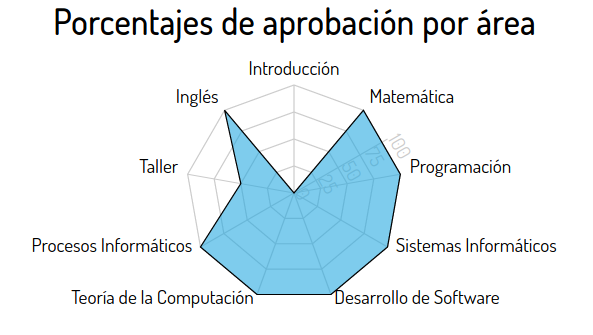
\includegraphics[scale=0.4]{images/seguimiento-academico/sa-porcentajesarea.png}
  \captionof{figure}{Porcentajes de aprobación por área}
  \label{fig:sa-porcentaje-area}
\end{figure}

\paragraph{Porcentajes de aprobacion por núcleo} \mbox{}\\
Radar

\begin{figure}[!htbp]
  \centering
    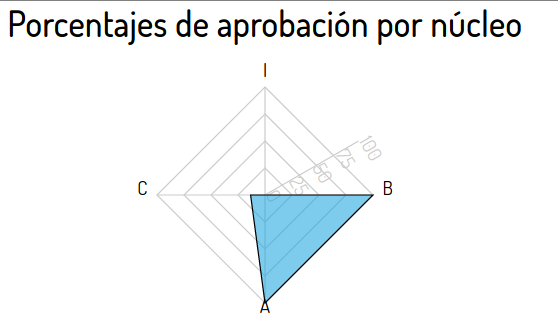
\includegraphics[scale=0.4]{images/seguimiento-academico/sa-porcentajesnucleo.png}
  \captionof{figure}{Porcentajes de aprobación por núcleo}
  \label{fig:sa-porcentaje-nucleo}
\end{figure}

\paragraph{Detalle de aprobación} \mbox{}\\
Tabla

\paragraph{Detalle de aprobación} \mbox{}\\
Gráfico de líneas
